% !TEX root = ./Thesis.tex

\chapter{Parahydrogen Induced Polarisation in a Microfluidic Device - PHIP on a Chip.}

The majority of the work in this chapter appears in \citep{eills2019high}

\section{Hyperpolarisation}

Was thinking to put Hyperpolarisation discussion here.
suggested order:
\begin{itemize}
  \item sensitivity - discussion of signal to noise and why Micro- is better in terms of mass
  sensitivity theory and equations
  \item What hyperpolarisation is - basic principles - where it's used
  \item Types of hyperpolarisation relevent - Description of DNP and Cryo-cooling "Brute force" method. Any more??
  \item Then the parahydrogen as it stands. Feel like it's missing something but can't put my finger on it.
\end{itemize}

\section{Sensitivity}\label{Sensitivity}

In \ref{Population} we saw how NMR has low polarisation levels governed by the boltzmann
distrubtion given in \eqn{eqn:Boltzmann}. For example, for a spin-1/2 particle in a static field of 14.1 Tesla
there is only a factor of $~6\times10^{-6}$ difference in the populations of the $\alpha$ and $\beta$ state.
Compared to other spectroscopic techniques NMR suffers from poor limits of detection (LODs). Raman Spectroscopy, has
LODs of $10^{-12}$ - $10^{-15}$, Laser indced flourescence (LIF) has detected concentrations at $10^{-13}$ and
mass spectrometry has achieved $10^{-19}$. All of which are several orders of magnitude higher than that of NMR.

\subsection{Signal Averaging}

In NMR, the signal that emerges from the probe contains uncontrolled random signals called noise as well
as the signal from the experiment. The most dominant source of noise comes from the thermal motions of the electrons
in the receiver coil. In order for the signal that originated from your sample to rise above the noise
signal averaging must be employed. This works as the sum of two identical experiments is twice the signal
of the orginal individual experiment:
\begin{equation}
  s_\text{NMR}(1+2) = s_\text{NMR}(1) + s_\text{NMR}(2) = 2s_\text{NMR}(1)
\end{equation}
The key is that this relationship doesn't apply equally to the noise which is random. A suitable
definition of the noise amplitude in a single experiment is given by the root mean square (RMS) noise defined
as:
\begin{equation}
  \sigma_\text{{noise}} = \langle~s_{\text{noise}}(1)^2\rangle^{1/2}
\end{equation}
where the angle bracket indicates an avergae over all sampling points. The RMS noise is the same for two
experiments assuming the noise is stationary i.e. the noise doesn't change from one experiment to the next.
However this does not imply that the noise from two experiments has twice the value. Summed over the two experiments
the RMS noise takes the value:
\begin{equation}
  \sigma_\text{{noise}}(1+2) \cong \sqrt{2}\sigma_{\text{noise}}(1)
\end{equation}
Since the noise over two experiments increases by $\sqrt{2}$ but the signal doubles we can write the signal to noise
ratio over two experiments as:
\begin{equation}
  \sqrt{2}\frac{s_{\text{NMR}}(1)}{\sigma_{\text{noise}}(1)}
\end{equation}
This can be extended to show the signal-to-noise over $N$ transients is a factor $\sqrt{N}$ larger than the
signal for a single transient. So by signal averaging over many scans the SNR can be increased.

 In principle this allows NMR signals that have a $<1$ SNR to be 'pulled out' of the noise. In reality this is
 time consuming as in order to repeat an experiment precisely it is essential to allow the spin sytem to
 reach thermal equilibrium again. The different NMR experiments must therefore be separated by an interval
 many times longer than $T_1$, which in some case can be several seconds. For example, if the SNR of the first
 experiment is 0.1 clearly the signal will be buried in the noise. The SNR maybe changed to 10:1 by signal averaging
 over 10,000 scans. If each scan takes 1 second this amounts to 3 hours of instrument time which is long but
 acceptable. However, if the SNR is 0.01 then it follows that 300 hours would now be needed which is not feasible.

 In order for smaller signals to be detected, the amount of signal i.e. the amount of polarisation in the sample,
 needs to be increased this can be done by preparing the sample in a specific way and is referred to as
 'hyperpolarisation'.

 \section{Hyperpolarisation}

As mentioned in \ref{Sensitivity} the polarisation levels of nuclear spins at room tempersture is low. In fact,
for protons it is only $3\times10^-6$ per tesla\citep{RN138}. The signal derived from an NMR experiment
is proportional to this polarisation and means that the sensitivty and LOD is limited. The highest
field avaiable commercially is ~28 tesla which corresponds to polarisaiton levels in protons of ~$10^-4$ and
whilst there are clear advantages to working in higher fields the size and more importanty the
cost make them unsuitable for many applications. Clearly just increasing the field is not a viable
option if we would like to acheive close to unity polarisation.

There are techniques for increasing the spin polarisation levels in samples to beyond the thermal
equilibrium. The general term used to describe these is hyperpolarisation. Hyperpolarisation has
applications in a diverse range of fields such as MRI \citep{RN139,RN140,RN151,RN152}, drug descovery
\citep{RN141,RN142}, reaction monitoring \citep{RN143,RN144,RN145}, metabolomics \citep{RN147,RN148},
catalysis\citep{RN149, RN150} and material chemistry \citep{RN153,piveteau2015structure,RN154}.

However, these hyperpolarised states are still subject to relaxation as discussed in \ref{Relaxation} and
return to thermal equilibrium with time constant $T_1$. This means the hyperpolarised spin order lasts seconds
to minutes which limits their applications.

\subsection{Techniques}

\subsubsection{Brute Force}

The most simple technique for hyperpolarisation is "brute force". It is performed by simply
cooling the sample to a few degrees kelvin in a high magnetic field \citep{RN155,RN157}. Under
these circumstances the polarisation of the nuclei is ~$1\%$. After sufficient time has passed
the sample is rapidly dissolved in a warm solvent in order to liberate the hyperpolarised
species as a solution for detection.

There are drawbacks however, firstly, long proton $T_1$ times at cryogenic temperatures means long
wait times are required in order to sufficiently build up polarisation in the sample. Secondly, and
perhaps more importantly, the limit of polarisation with this technique is around $10^-2$ at acheivable
magnetic fields and temperatures.

\subsubsection{Dynamic Nuclear Polarisation}

Several different types of dynamic nuclear polarisation (DNP) have been reported. These are solution
state DNP\citep{RN158}, solid state magic angle spinning (MAS) DNP\citep{RN159} and static solid state DNP with
dissolution and observation\citep{RN160}. This type is referred to as dissoltuion-DNP and written as d-DNP.

d-DNP uses the thermal equilibrium electron spin polarisation to polarize the nuclei under investigation. Unity
polarization of the elctrons is acheived by cooling to cryogenic temperatures (<2K) in a high magnetic field (>7T).
The electron polarization is transferred to nearby nuclear spins by saturating microwave frequency radiation.

 The source of the electrons are 'free radicals' - molecules that have an unpaired elctron spin, that
 are spread homogeneously throughout the sample after cooling the sample is held in a cryostat which is at
 1.2-1.5K. The electrons have a much shorter $T_1$ in contrast to nuclear spins so after irradiation with
 microwave radiation to induce polarization transfer between elctrons and nuclei, the electrons repolarise
 quickly compared to the nuclei who retain non-equilibrium polarization. This polarization diffuses throughout the
 sample. After some time, tens of minutes is not uncommon, the nuclear spins are polarised to around 0.1. The
 sample is then rapidly dissolved with a pressurised hot solvent into seperate high field magnet for detection.

 The large equipment required for d-DNP, as well as the high cost of liquid helium for the cryostat and
 the superconducting magnets make this method quite prohibitive. Very few groups could do d-DNP with little
 overhead equipment costs.

\section{Parahydrogen Iduced Polarisation - PHIP}

\subsection{Porduction of Parahydrogen}

Hydrogen exists as a diatomic made up of two protons and two electrons. As such, the total
wave function contains electronic, vibrational, rotational and spin components and can be
written as:

\begin{equation}
 \Psi^{tot} =\Psi^{elec}\Psi^{vib}\Psi^{rot}\Psi^{spin}
\end{equation}

Because the two protons are fermions they are subject to the Pauli exclusion principle
which states that: the total wave function must be antisymmetric with respect to exchange. With
this is mind, it is important to note that the electronic and vibrational states are symmetrical in the ground state and if we assume that they occupy the ground state, we find that the symmetry of the overall wave function deoends of the symmetry of $\Psi^{rot}$$\Psi^{spin}$.

Rotational wavefunctions have quantum number J. For even numbers of J (J=0,2...) the wavefunction is symmetric with respect to particle exchange for odd numbers of J (J=1,3...) the wavefunction is antisymmetric. The nuclear spin wave function can also be symmetric or antisymmetric. By adding the angular momentum of both spins it can be shown that they combine to give four possible wavefunctions
they are:

\begin{align}
\Psi_{1}^{T+} =& \ket{\alpha\alpha}\\
\Psi_{1}^{T0} =& \frac{1}{\sqrt{2}} (\ket{\alpha\beta}+\ket{\beta\alpha})\\
\Psi_{1}^{T-} =& \ket{\beta\beta}\\
\Psi_{0}^{S0} =& \frac{1}{\sqrt{2}} (\ket{\alpha\beta}-\ket{\beta\alpha})
\end{align}

The three triplet ($T$) states have spin quantum number I = 1 and are symmetric with respect to spin exchange whilst
the singlet ($S$) state has I = 0 and is antisymmetric. Hydrogen in the triplet state is refered to as ortho and the
singlet state is referred to as para.

In order for $\Psi^{tot}$ to be antisymmetric the antisymmetric rotational states need to be coupled with the symmetric (triplet) spin states whilst the symmetric rotational states should couple with the antisymmetric (singlet) state.

The rotational energy is given by $E_j = \frac{J(J+1)\hbar^2}{2I}$
where I is the moment of inertia of the diatomic and is given by $I = \mu l^2$, where $\mu$ is the reduced mass,
and $l$ is the internuclear distance.

\begin{figure*}
  \begin{center}
  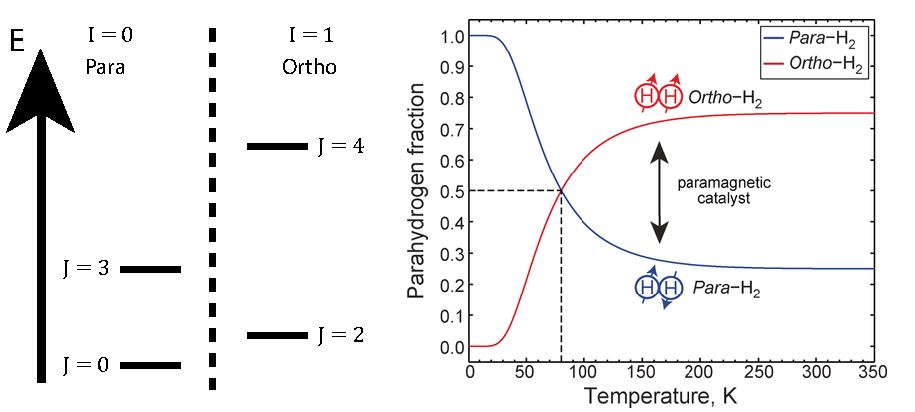
\includegraphics[width=\textwidth]{Para-OrthoH2.pdf}
  \end{center}
  \caption{Left: The rotational energy levels of para- and orthohydrogen with their associated J values. Right: a graph
  showing the fraction of para- and orthohydrogen as a function of temperature. The dotted line shows 50\% para
  enrichment that is acheived by cooling to 77K using liquid nitrogen. Image taken from \citep{barskiy2017nmr}.}
  \label{fig:POH2}
\end{figure*}


At room temperature the ratio of ortho to para hydrogen is 3 to 1. However, by cooling down hydrogen the lowest (J = 0, 1) rotational enrgy states start to become populated so too do the corresponding spin states. By cooling alone the ratio would remain unchanged. One can't convert from ortho to para spin states without the aid of a catalyst (typically charcoal or iron (III) oxide). The catalyst temporarily breaks the symmetry of the \ce{H_2} molecule and allows these spin-spin transitions and allows the pure para- form of hydrogen to be produced. Crucially, when warmed up to
room temperature in the absence of a symmetery breaking catalyst, no conversion from the singlet state $S_0$ back to
the triplet states $T_+$, $T_0$, $T_-$ occurs. This is because the nuclear spin flip required would not
conserve angular momentum and is therefore disallowed. It therefore possible to store pure parahydrogen
in the right container for days to weeks.

Para enrichment fraction, $f$, can be measured by NMR. By measuring the o\ce{H_2} signal of the enriched \ce{H_2} ($S_{e}$) and comparing it to the signal obtained from the same amount of \ce{H_2} at room temperature ($S_{rt}$). The enrichment fraction is given by[\citep{RN131, RN132}:

\begin{equation}\label{pfrac}
  f = 1 -(3S_{e}/4S_{rt})
\end{equation}

\subsection{PASADENA and ALTADENA}\label{PASADENA and ALTADENA}

Parahydrogen and synthesis allow dramatically enhanced nuclear alignment (PASADENA)[\citep{RN129} and adiabatic longitudinal transport after dissocciation engenders net alignment (ALTADENA)[\citep{RN128}
 are subclasses of PHIP experiments characterised by the strength of magnetic
field in which the hydrogenation and detection are performed.

The difference between PASADENA and ALTADENA are the J-coupling regimes in which the reaction and detection happen. In PASADENA experiments the reaction and detection is carried out at high field (>1 T) whereas in
ALTADENA, the reaction is carried out at low field (< 10 mT), and the product is transferred to a high magnetic field for detection\citep{RN130}.

This difference manifests itself as a difference in J-coupling regimes in the parahydrogen derived hydrogens in the product molecule. ALTADENA refers to hydrogens in the stong regime and PASADENA refers to the weak regime. The strength of regime is determined by the value of the J-coupling (in Hz) compared to the value of the difference in chemical shifts of the individual protons.
A strong regime has J-coulings that take the approxiamte value of the difference in chemical shift ($\frac{\delta{\omega}}{J}\approx1$). A weak regime has J-couplings much smaller than the difference in chemical shift ($\frac{\delta{\omega}}{J}>>1$). Since the chemical shift depends on external magnetic field ($B_{0}$) and the J-couplings are independent of field one can select an appropriate magnetic field for the desired experiment.

\subsubsection{Spin Physics}

The spin physics of these types of hydrogenative PHIP are
accessible through the density operator formulism.

In a PASADENA type experiment, parahydrogen is then added to molecule in high field forming a weakly coupled AX
system of the type discussed in \ref{PASADENA and ALTADENA}. Due to the weak coupling, $\frac{\delta{\omega}}{J}>>1$, the eigenbasis is close to the Zeeman basis. The initial density operator, $\hat{\rho}_{\text{ini}}$ From our earlier
definitions this is:
\begin{equation}
  \hat{rho}_{\text{ini}} = \ket{\Psi_{0}^{S}}\bra{\Psi_{0}^{S}} = \frac{1}{2}\ket{\alpha\beta -
  \beta\alpha}\bra{\alpha\beta - \beta\alpha}
\end{equation}

using the zeeman basis states for a 2 spins system described in SPINSTATES

\begin{align}
  \hat{\rho}_{\text{ini}}\quad=& \frac{1}{2} \begin{pmatrix}
  0\\
  1\\
  -1\\
  0
  \end{pmatrix} \otimes \begin{pmatrix}
    0 & 1 & -1 & 0
    \end{pmatrix}\\
  =& \frac{1}{2}\begin{pmatrix}
  0 & 0 & 0 & 0\\
  0 & 1 & -1 & 0\\
  0 & -1 & 1 & 0\\
  0 & 0 & 0 & 0
\end{pmatrix} \\
\end{align}

These diagonal elements (populations) do not evolve as these components commute with the Hamiltonian. The off-diagonal
elements (coherences) evolve at a rate $\approx\delta{v}$.

As the reaction continues an ensemble of molecules that are hydrogenated at different time points, this gives
a new density operator, $\hat{\rho}_pr$, expressed as:
\begin{equation}
  \hat{\rho}_{\text{pas}} = \frac{1}{t} \int_t=0^t{\text{exp}\{-i\hat{H}t\}\hat{\rho}_{\text{ini}}\text{exp}\{+i\hat{H}t\}}dt
\end{equation}
Usually, the hydrogenation period is much longer than the coherence evolution. These average to zero and so the
density operator becomes:
\begin{equation}
  \hat{\rho}_{\text{pas}} = \frac{1}{2}\begin{pmatrix}
  0 & 0 & 0 & 0\\
  0 & 1 & 0 & 0\\
  0 & 0 & 1 & 0\\
  0 & 0 & 0 & 0
\end{pmatrix}
\end{equation}

\fig{fig:PASADENA} shows the eigensate populations and general simulated spectra of a thermal equilibrium experiment and
a PASADENA experiment.

In a usual NMR spectra a $\pi/2$ pulse is used to excite observable single quantum coherences. For a PASADENA signal to
be observed, a $\frac{\pi}{4}$ pulse must be used. The reason becomes clear when $\hat{\rho}_{\text{pr}}$ is rewritten
in terms of angular momentum operators, neglecting the identity matrix this is:
\begin{equation}
  \hat{\rho}_{\text{pas}} = -\hat{I}_{1z}\hat{I}_{2z}
\end{equation}
a $\frac{\pi}{2}$ pulse has the following effect:
\begin{equation}
  \hat{\hat{R}}_y(\frac{\pi}{2})\hat{\rho}_{\text{pas}} = -\hat{I}_{1x}\hat{I}_{2x}
\end{equation}

which is an unobservable doube quantum cohenrence nd the reason pure parahydrogen is NMR silent. However,
a $\pi/4$ $y$-pulse gives:
\begin{equation}
\hat{\hat{R}}_y(\frac{\pi}{4})\hat{\rho}_{\text{pas}} = -\frac{1}{2}(\hat{I}_{1x}\hat{I}_{2x} + \hat{I}_{1x}\hat{I}_{2z} + \hat{I}_{1z}\hat{I}_{2x} + \hat{I}_{1z}\hat{I}_{2z})
\end{equation}

\begin{figure*}
  \begin{center}
  \includegraphics[width=0.7\columnwidth,height=7cm,keepaspectratio]{Pasadena-population-Balls.pdf}
  \end{center}
  \caption{Above: Populations of states represented as balls in a thermal (left) and a PASADENA experiment. Below: Simulations of spectra arising from adding thermal hydrogen to a molecule (left) and of a PASADENA experiment when adding parahydrogen.}
  \label{fig:PASADENA}
\end{figure*}

In an ALTADENA exeriment, the hydrogenation is performed at low field. In this case, when a molecule of hydrogen
is added to a substrate the denstiy operator ,$\hat{\rho}_\text{ini}$, is projected onto the new eigenbasis which
at low field (where $\frac{\delta{\omega}}{J}<<1$) is the singlet-triplet basis. To a good approximation the only term is the $\ket{S_0}$ and there is no evolution of the system.

The sample is then transferred to high-field (where $\frac{\delta{\omega}}{J}>>1$). It is done adiabatically, this is defined as the rate of change of magnetic field being small with respect to $(J_{12})^2$. As the field increases, the eigenbasis changes from singlet-triplet to the Zeeman basis. The adiabatic change carries the population of the $\ket{S_0}$ state to the $\ket{\alpha\beta}$ state this is shown graphically in \fig{fig:SingletTriplet} In this case, only one of the four energy levels, namely $\alpha\beta$ is now populated, therefore the density operator, $\hat{\rho}_{alta}$ is given by:
\begin{equation}
  \hat{\rho}_{\text{alta}} = \ket{\alpha\beta}\bra{\alpha\beta}
\end{equation}
 This leads to \citep{RN128}:
\begin{equation}
  \hat{\rho}_{\text{alta}} = \hat{I}_{1z}\hat{I}_{2z}±(\hat{I}_{1z}-\hat{I}_{2z})
\end{equation}

\begin{figure}
  \begin{center}
  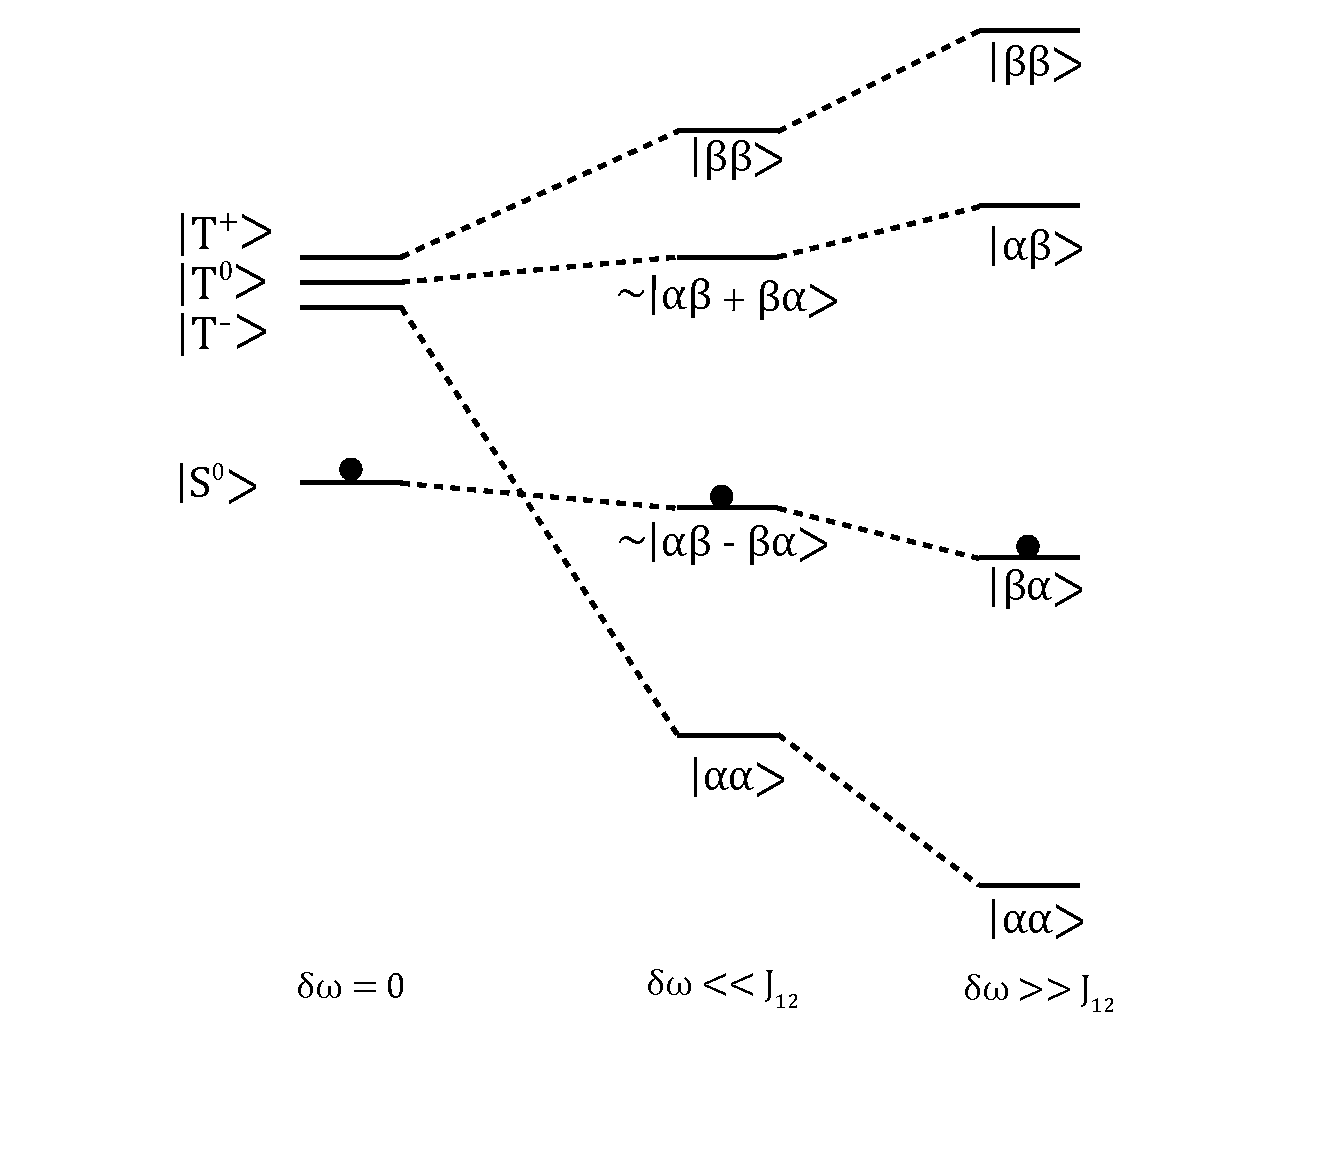
\includegraphics[width=0.7\columnwidth,height=7cm,keepaspectratio]{ALTADENA-overview.pdf}
  \end{center}
  \caption{Correlation diagram for the ALTADENA effect. Hydrogenation at low field populates the singlet state, adiabatically icreasing the field carries the population into a high field state.}
  \label{fig:SingletTriplet}
\end{figure}

The result of a $\pi/4$ pulse along the $y$-axis yields:
\begin{equation}
  \hat{\hat{R}}_y(\frac{\pi}{2})\hat{\rho}_{\text{alta}} = \frac{1}{2}(\hat{I}_{1z}\hat{I}_{2x})±\frac{1}{2\sqrt{2}}(\hat{I}_1x-\hat{I}_2x)
\end{equation}
This gives rise to the two out of phase doublets that are typical for an ALTADENA experiment on an AX system. A diagram
is provided in \fig{fig:ALTADENA} that shows a simulated spectra compared to a thermal spectrum.

\begin{figure}
  \begin{center}
  \includegraphics[width=\columnwidth,height=7cm,keepaspectratio]{Altadena-Population-Balls.pdf}
  \end{center}
  \caption{Above: Populations of Zeeman states represented by balls for thermal(left) and ALTADENA(right) experiments.
  Below: Simulations of a thermal spectrum after applying a $\pi/4$ pulse and an ALTADENA experiment.}
  \label{fig:ALTADENA}
\end{figure}
